\chapter{Test Problem}
\label{chap:testprob}

This section describes a simple test problem which was used to calculate $\delta R$ for various perturbations.

%%%%%%%%%%%%%%%%%%%%%%%%%%%%%%%%%%%%%%%%%%%%%%%%%%%%%%%%%%%%%%%%%%%%%%%%%%%%%%%%
\section{Test Problem Overview}
\label{sec:bg:tp:overview}
%%%%%%%%%%%%%%%%%%%%%%%%%%%%%%%%%%%%%%%%%%%%%%%%%%%%%%%%%%%%%%%%%%%%%%%%%%%%%%%%

The test problem consists of an accelerator-based DD fusion (around 2.45 MeV) neutron source, a tally region in which it is desired to maximize the ${}^{235}\text{U}$ fission rate, a moderating region, and a steel wall to separate the moderator from the tally region.
The goal of the test problem is to use the equation for $\delta R$ to find the moderating material that results in the highest response in the tally.
Water was chosen as the baseline moderating material.
A diagram of the test problem geometry is shown in Figure \ref{fig:testprob:material_map}.

\begin{figure}[h!]
  \centering
  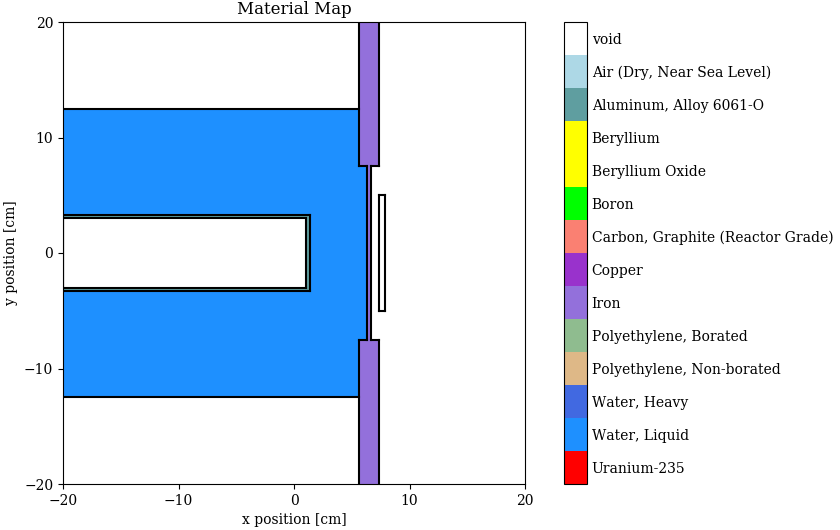
\includegraphics[width=\linewidth]{content/testprob/material_map.png}
  \caption{Material map for test problem.}
  \label{fig:testprob:material_map}
\end{figure}

The geometry is entirely comprised of rectangular parallelepipeds (RPPs in MCNP) to avoid there being mesh elements with mixed materials.
In ADVANTG, the 3D spatial mesh has 43 elements in the x-direction and 44 elements in both the y- and z-directions for a total of 83,248 voxels.

The ``27n19g'' multigroup cross section library, which contains 27 neutron energy groups and 19 gamma energy groups, was used.
Since the first two neutron energy groups in this library are above 2.45 MeV, they are unused, leaving 25 neutron energy groups.
Since the tally is a neutron tally and the library does not account for photonuclear reactions, all of the gamma groups are also unused, leaving 25 total energy groups.
Upscattering was explicitly turned off for this analysis to decrease computation time.

The quadrupole range quadrature set with an order of 10 was used.
There were 4 azimuthal and 4 polar directions per octant, for a total of 16 directions per octant, or 128 directions overall.

The forward angular flux thus has $83,248 \times 25 \times 128 = 266,393,600$ values.
Even in this small test problem, the angular forward and adjoint fluxes take up about 4 GB of storage space.

The locations of the energy-integrated source and responses are shown in Figures \ref{fig:testprob:source_total} and \ref{fig:testprob:response_total}.
The source and response energy spectra are shown in \ref{fig:testprob:spectra_lin}.
The source energy spectrum is spans the range between 1.97 and 3.23 MeV.
The response energy spectrum is equivalent to the ${}^{235}\text{U}$ fission cross section, which is highest at thermal energies.

\begin{figure}
  \centering
  \begin{minipage}{0.49\linewidth}
    \centering
    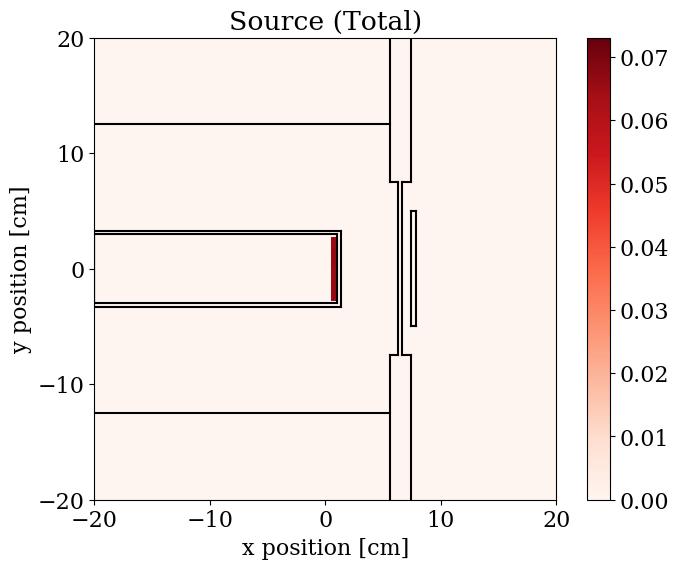
\includegraphics[width=\linewidth]{content/testprob/source_total.png}
    \caption{Location of energy-integrated source in test problem.}
    \label{fig:testprob:source_total}
  \end{minipage}
  \hfill
  \begin{minipage}{0.49\linewidth}
    \centering
    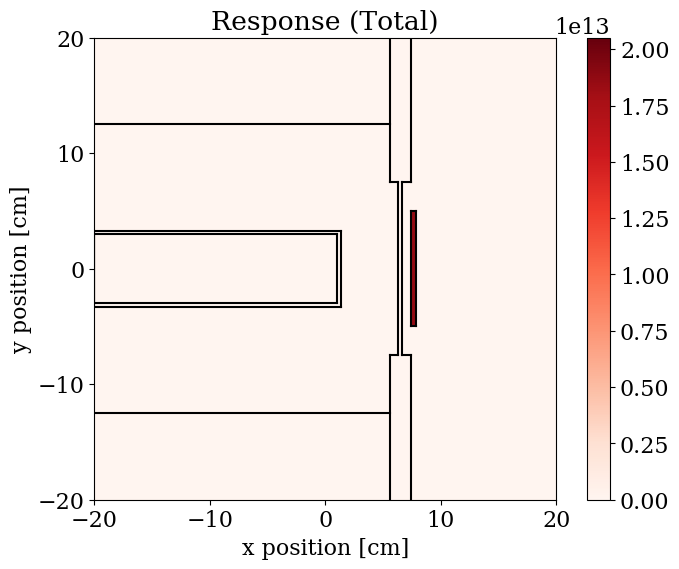
\includegraphics[width=\linewidth]{content/testprob/response_total.png}
    \caption{Location of energy-integrated response in test problem.}
    \label{fig:testprob:response_total}
  \end{minipage}
\end{figure}
\begin{figure}
  \centering
  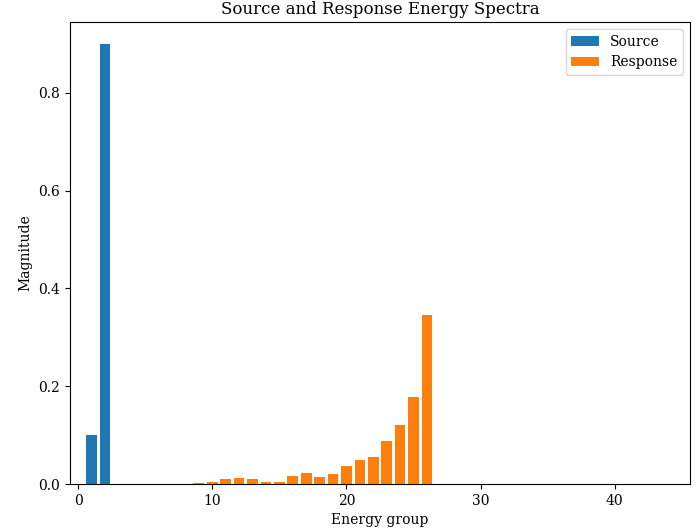
\includegraphics[width=0.5\linewidth]{content/testprob/spectra_lin.png}
  \caption{Source and response energy spectra in test problem.}
  \label{fig:testprob:spectra_lin}
\end{figure}

%%%%%%%%%%%%%%%%%%%%%%%%%%%%%%%%%%%%%%%%%%%%%%%%%%%%%%%%%%%%%%%%%%%%%%%%%%%%%%%%
\section{Flux in Test Problem}
\label{sec:bg:tp:flux}
%%%%%%%%%%%%%%%%%%%%%%%%%%%%%%%%%%%%%%%%%%%%%%%%%%%%%%%%%%%%%%%%%%%%%%%%%%%%%%%%

% Note: first energy group should actually be group 1, not group 2.

The scalar forward flux for energy groups 2 (1.8268 to 3.0119 MeV) and 26 ($10^{-11}$ to $10^{-8}$ MeV) are shown in Figures \ref{fig:testprob:scalar_flux_fwd_g02} and \ref{fig:testprob:scalar_flux_fwd_g26}.
The group 2 flux shows that high-energy neutrons radiate out from the source.
Ray effects, which are caused by the angular discretization, are clearly visible in this plot.
The group 26 flux shows that the thermal neutron population is significantly more spread out, existing as a cloud that encompasses most of the moderating region.

\begin{figure}
  \begin{minipage}{0.49\linewidth}
    \centering
    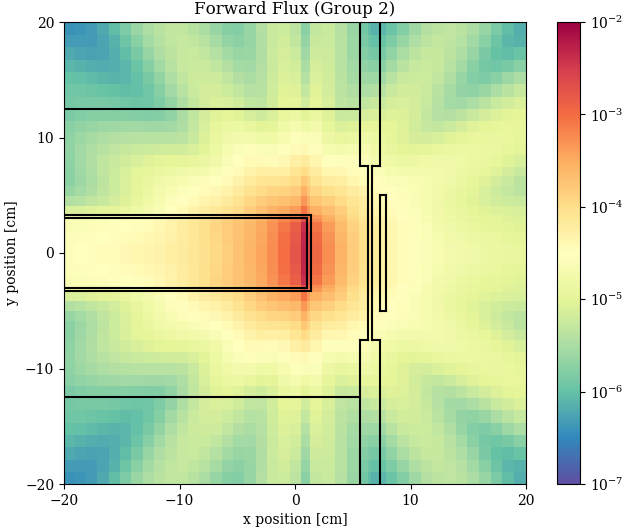
\includegraphics[width=\linewidth]{content/testprob/scalar_flux_fwd_g02.png}
    \caption{Scalar forward flux in energy group 2 in test problem.}
    \label{fig:testprob:scalar_flux_fwd_g02}
  \end{minipage}
  \hfill
  \begin{minipage}{0.49\linewidth}
    \centering
    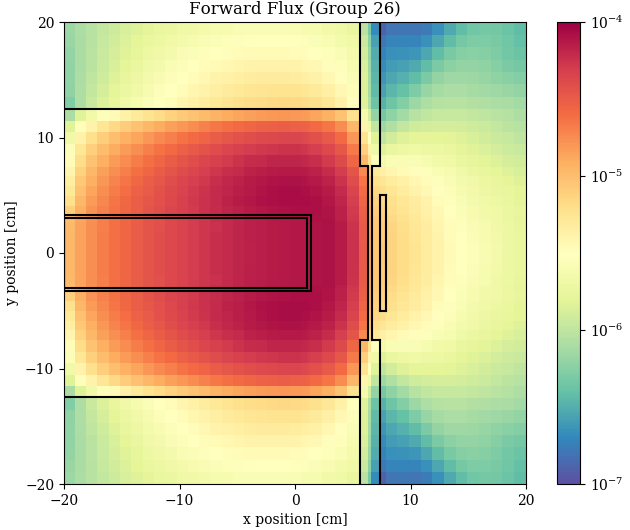
\includegraphics[width=\linewidth]{content/testprob/scalar_flux_fwd_g26.png}
    \caption{Scalar forward flux in energy group 26 in test problem.}
    \label{fig:testprob:scalar_flux_fwd_g26}
  \end{minipage}
\end{figure}

The scalar angular flux for energy groups 2 and 26 are shown in Figures \ref{fig:testprob:scalar_flux_adj_g02} and \ref{fig:testprob:scalar_flux_adj_g26}.
The group 26 adjoint flux shows that thermal neutrons close to the detector have a high likelihood of contributing to the detector.
The group 2 adjoint flux shows that fast neutrons have the highest likelihood of contributing to the detector while they are still in the moderating region.
This is because they are more likely to scatter down to thermal energies and then contribute to the detector than they are to immediately contribute to the detector as fast neutrons.

\begin{figure}
  \begin{minipage}{0.49\linewidth}
    \centering
    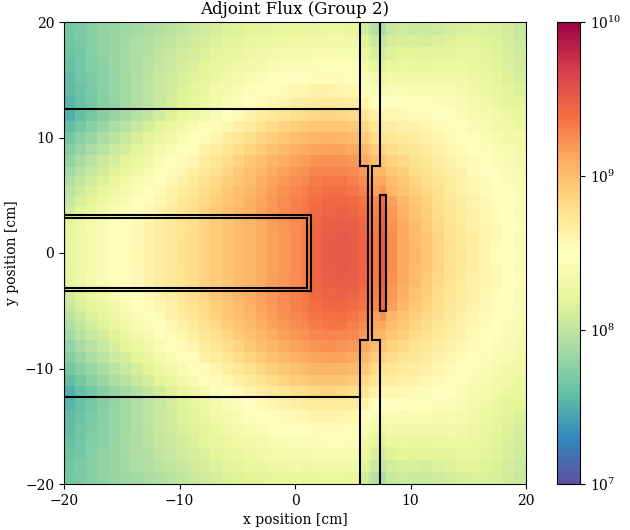
\includegraphics[width=\linewidth]{content/testprob/scalar_flux_adj_g02.png}
    \caption{Scalar adjoint flux in energy group 2 in test problem.}
    \label{fig:testprob:scalar_flux_adj_g02}
  \end{minipage}
  \hfill
  \begin{minipage}{0.49\linewidth}
    \centering
    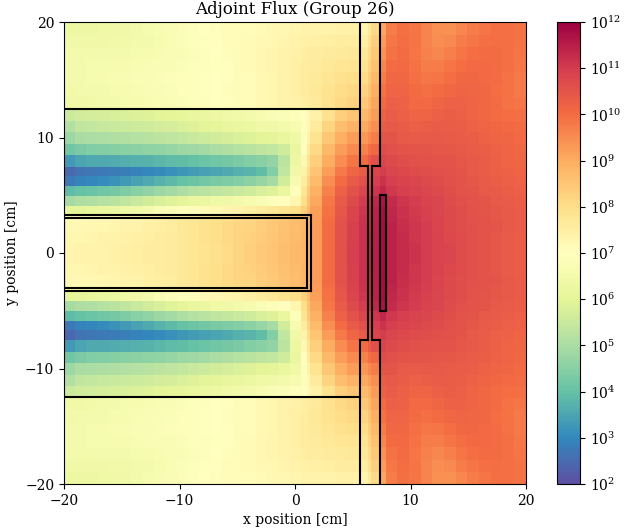
\includegraphics[width=\linewidth]{content/testprob/scalar_flux_adj_g26.png}
    \caption{Scalar adjoint flux in energy group 26 in test problem.}
    \label{fig:testprob:scalar_flux_adj_g26}
  \end{minipage}
\end{figure}

The contributon flux for energy groups 2 and 26 are shown in Figures \ref{fig:testprob:scalar_flux_con_g02} and \ref{fig:testprob:scalar_flux_con_g26}.
The energy-integrated contributon flux is shown in Figure \ref{fig:testprob:scalar_flux_con_total}.
The contribution flux is the result of taking the product of the forward and adjoint \textit{angular} fluxes and the integrating over angle.
Since the region on the right side of the problem is void, all forward particles in that region are traveling to the right, and all adjoint particles in that region are traveling to the left.
Thus, the contributon in that region is zero.
The contributon flux is at its highest in the region in between the source and detector, which makes sense intuitively.

\begin{figure}
  \begin{minipage}{0.49\linewidth}
    \centering
    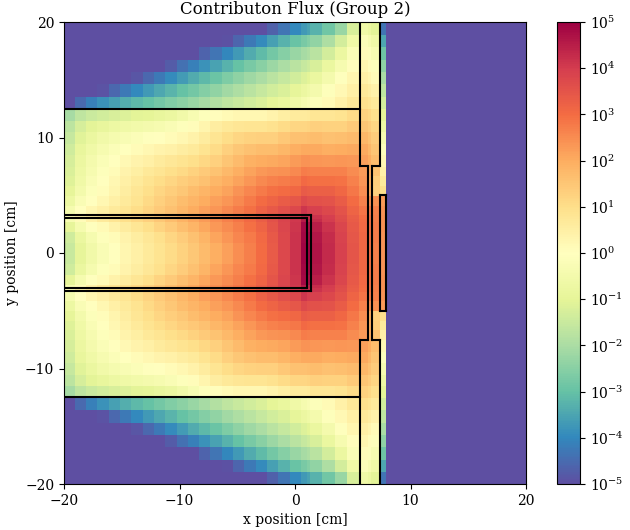
\includegraphics[width=\linewidth]{content/testprob/scalar_flux_con_g02.png}
    \caption{Contributon flux in energy group 2 in test problem.}
    \label{fig:testprob:scalar_flux_con_g02}
  \end{minipage}
  \hfill
  \begin{minipage}{0.49\linewidth}
    \centering
    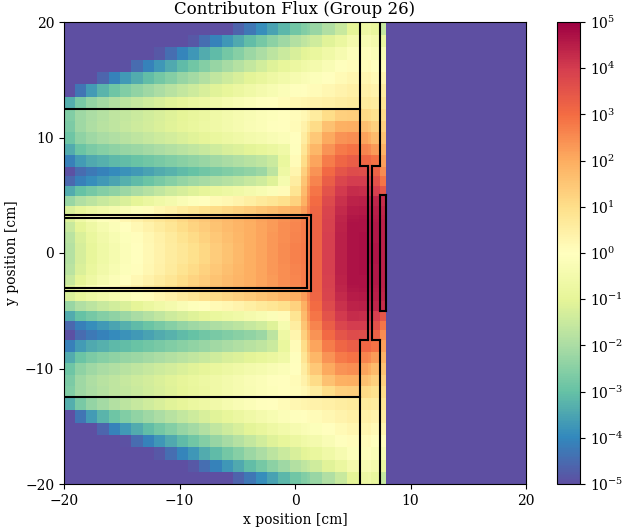
\includegraphics[width=\linewidth]{content/testprob/scalar_flux_con_g26.png}
    \caption{Contributon flux in energy group 26 in test problem.}
    \label{fig:testprob:scalar_flux_con_g26}
  \end{minipage}
\end{figure}
\begin{figure}
  \centering
  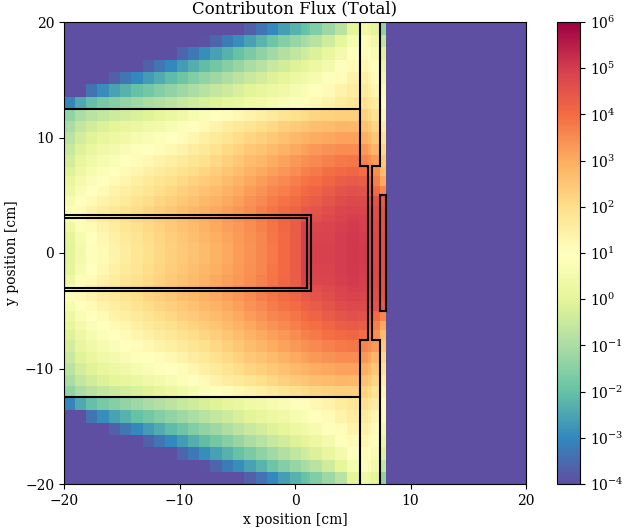
\includegraphics[width=0.5\linewidth]{content/testprob/scalar_flux_con_total.png}
  \caption{Energy-integrated contributon flux in test problem.}
  \label{fig:testprob:scalar_flux_con_total}
\end{figure}

The forward current for energy groups 2 and 26 are shown in Figures \ref{fig:testprob:current_fwd_g02} and \ref{fig:testprob:current_fwd_g26}.
The forward current shows the net directionality of the forward flux.
Fast neutrons radiate outward from the source.
The thermal flux is highly isotropic inside the moderator, but it is highly directional in the void because neutrons can only leave the moderator to the right with no ability to re-enter.

\begin{figure}
  \begin{minipage}{0.49\linewidth}
    \centering
    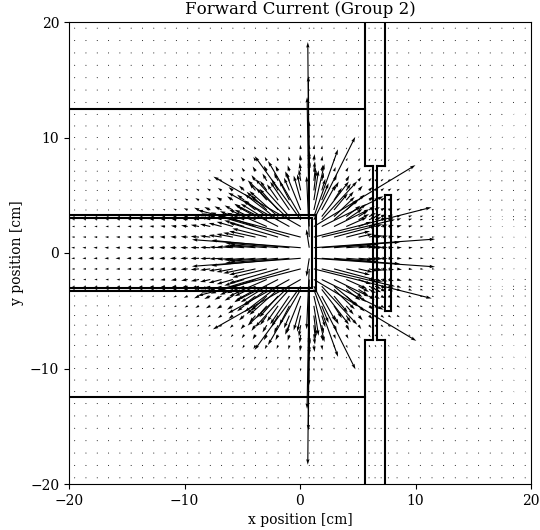
\includegraphics[width=\linewidth]{content/testprob/current_fwd_g02.png}
    \caption{Forward current in energy group 2 in test problem.}
    \label{fig:testprob:current_fwd_g02}
  \end{minipage}
  \hfill
  \begin{minipage}{0.49\linewidth}
    \centering
    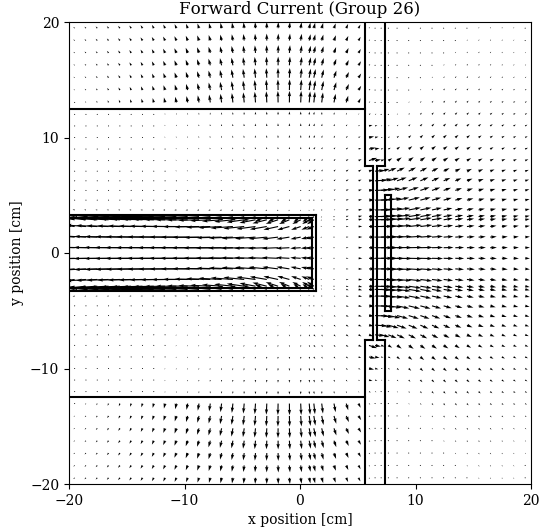
\includegraphics[width=\linewidth]{content/testprob/current_fwd_g26.png}
    \caption{Forward current in energy group 26 in test problem.}
    \label{fig:testprob:current_fwd_g26}
  \end{minipage}
\end{figure}

The adjoint current for energy groups 2 and 26 are shown in Figures \ref{fig:testprob:current_adj_g02} and \ref{fig:testprob:current_adj_g26}.
The adjoint current shows the net directionality of the adjoint flux.
Adjoint fast neutrons do not show strong directionality.
Adjoint thermal neutrons radiate outward from the detector.

\begin{figure}
  \begin{minipage}{0.49\linewidth}
    \centering
    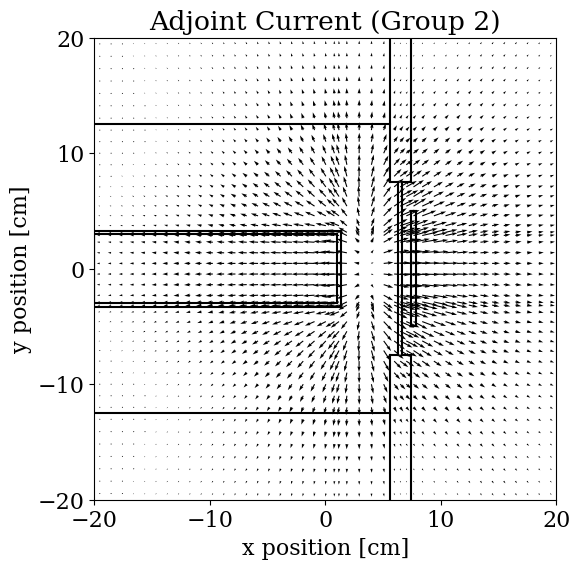
\includegraphics[width=\linewidth]{content/testprob/current_adj_g02.png}
    \caption{Adjoint current in energy group 2 in test problem.}
    \label{fig:testprob:current_adj_g02}
  \end{minipage}
  \hfill
  \begin{minipage}{0.49\linewidth}
    \centering
    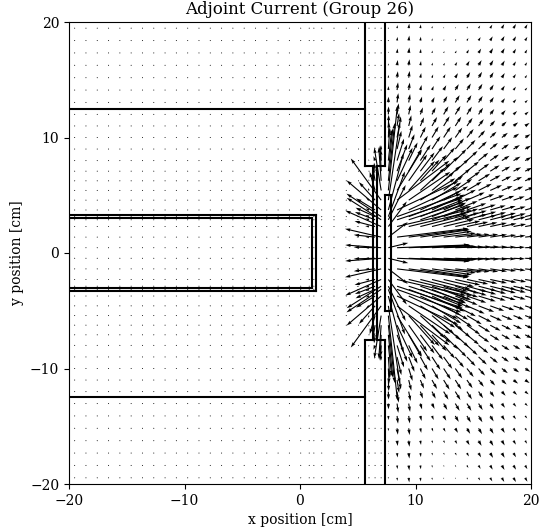
\includegraphics[width=\linewidth]{content/testprob/current_adj_g26.png}
    \caption{Adjoint current in energy group 26 in test problem.}
    \label{fig:testprob:current_adj_g26}
  \end{minipage}
\end{figure}

%%%%%%%%%%%%%%%%%%%%%%%%%%%%%%%%%%%%%%%%%%%%%%%%%%%%%%%%%%%%%%%%%%%%%%%%%%%%%%%%
\section{Calculation of $\delta R$ in Test Problem}
\label{sec:bg:tp:dr}
%%%%%%%%%%%%%%%%%%%%%%%%%%%%%%%%%%%%%%%%%%%%%%%%%%%%%%%%%%%%%%%%%%%%%%%%%%%%%%%%

% Table \ref{tab:testprob:mats} shows an example table.
%
% \begin{table}[h]
%   \centering
%   \caption[Short table caption]{Long table caption}
%   \label{tab:testprob:mats}
%   \begin{tabular}{| c | c | c |}
%     \hline
%     \textbf{Material ID} & \textbf{Material} \\ \hline
%      0 & Void                 \\ \hline
%      1 & Air                  \\ \hline
%      2 & Aluminum             \\ \hline
%      3 & Beryllium            \\ \hline
%      4 & Beryllium oxide      \\ \hline
%      5 & Boron                \\ \hline
%      6 & Graphite             \\ \hline
%      7 & Copper               \\ \hline
%      8 & Iron                 \\ \hline
%      9 & Borated polyethylene \\ \hline
%     10 & Polyethylene         \\ \hline
%     11 & Heavy water          \\ \hline
%     12 & Light water          \\ \hline
%     13 & Uranium-235          \\ \hline
%   \end{tabular}
% \end{table}
